\documentclass[12pt, a4paper, notitlepage]{report}
\usepackage{mathptmx}
\usepackage[T1]{fontenc}
\usepackage[utf8x]{inputenc}
\usepackage[english]{babel}
\usepackage{graphicx}
\usepackage{float}
\usepackage{amsmath}
\usepackage{mathtools}
\usepackage{amsfonts}
\usepackage{enumerate}
\usepackage[caption = false]{subfig}
\usepackage[top=2.5cm, bottom=2.5cm, left=2cm, right=2cm]{geometry}
\usepackage[font={small,it}]{caption}
\usepackage{fancyhdr}
\usepackage{listings}
\usepackage{color}

\graphicspath{ {./Comp\_1000/} {./Comp\_1500/} {./Comp\_2000/} {./Real\_1000/} {./Real\_1500/} {./Real\_2000/} }

\definecolor{dkgreen}{rgb}{0,0.6,0}
\definecolor{gray}{rgb}{0.5,0.5,0.5}
\definecolor{mauve}{rgb}{0.58,0,0.82}
\definecolor{lyellow}{rgb}{1,1,0.9}

\lstset{backgroundcolor=\color{lyellow},
	frame=tb,
	language=Fortran,
	aboveskip=3mm,
	belowskip=3mm,
	showstringspaces=false,
	columns=flexible,
	basicstyle={\small\ttfamily},
	numbers=none,
	numberstyle=\tiny\color{gray},
	keywordstyle=\color{blue},
	commentstyle=\color{dkgreen},
	stringstyle=\color{mauve},
	breaklines=true,
	breakatwhitespace=true,
	tabsize=3
}

\pagestyle{fancy}
\lhead{Tommaso Tabarelli}
\chead{\thepage}
\rhead{\today}
\cfoot{Information theory and computation}
\rfoot{A.y. 2019/2020}
\lfoot{Exercise 5}

\begin{document}

\begin{center}
	\LARGE{Quantum information and computation: homework 5}\\
	\Large{of Tommaso Tabarelli}
\end{center}


\begin{abstract}
	In this homework we are asked to analyze some random matrices properties and check results match with theoretical expectations. We shall do it using \textit{Fortran} executables to create matrices and store the normalized differences between their eigenvalues, collect the results with \textit{Python} and fit results using \textit{Gnuplot}.
\end{abstract}

\section*{Theory}
In probability theory and mathematical physics, a random matrix is a matrix-valued random variable; that is, a matrix in which some or all elements are random variables. Many important properties of physical systems can be represented mathematically as matrix problems.\\
Usually to generate random matrices gaussian distributed values are used. In general, matrix can have complex values.\\
Most analyzed matrices are \textit{hermitian} ones and symmetric real ones. From the ordered eigenvalues $\lambda_1,\lambda_2,...,\lambda_n,...$ normalized spacings $s = \frac{(\lambda_{i+1} - \lambda_{i})}{\langle (\lambda_{i+1} - \lambda_{i} \rangle} $ can be defined.\\
The general spacing distribution has the form:
$$ P(s) = a \cdot s^\alpha \cdot e^{-b \cdot s^\beta} $$

The theoretical parameters for the hermitian matrix spacing distribution are:
\begin{table}[H]
	\centering
	\begin{tabular}{|c|c|}

	\hline
	
	a			& 32 / $\pi^2$ $\simeq 3.243$ 	\\
	$\alpha$	& 2				\\
	b			& 4 / $\pi$	$\simeq 1.273 $	\\
	$\beta$		& 2				\\
	
	\hline

	\end{tabular}
\end{table}

while for gaussian distributed real eigenvalues (the way the "symmetric real matrix" is built) they are not know due to the way we construct them.


\section*{Code development}
To begin with, a \textit{random number generator} (RNG) module was created to be included in Fortran program. It implements Box-Muller algorithm which generates gaussian distributed random numbers starting from built-in uniform r.n.g. \textit{RANDOM\_NUMBER}.

\begin{lstlisting}
MODULE RNG
	! Module to generate Normal random number
	IMPLICIT NONE
	
	INTERFACE Normal_rng
		MODULE PROCEDURE Normal_rng_comp8
	END INTERFACE Normal_rng
	
	CONTAINS
	SUBROUTINE Normal_rng_comp8(x, y)
		REAL*8 :: u1, u2, r, theta
		REAL*8, INTENT(OUT) :: x, y
		
		CALL RANDOM_NUMBER(u1)
		CALL RANDOM_NUMBER(u2)
		
		r = SQRT(2*(-LOG(u1)))
		! pi = 2*arcsin(1)
		theta = 2*(2*ASIN(1.)) * u2
		
		x = r*COS(theta)
		y = r*SIN(theta)
	
	END SUBROUTINE Normal_rng_comp8

END MODULE RNG
\end{lstlisting}

This module is used to initialize all values of hermitian and "real" diagonal matrices.\\
The choice was to use two different files for hermitian matrix and gaussian ones. In both, alternative spacings are read from file at beginning and utility variables are defined (for examples, \textit{lapack}'s subroutines need some variables to store output that are not interesting for our pourposes).\\
In the first program, hermitian matrix is initialized using \textit{RNG}'s \textit{Normal\_rng} subroutine, \textit{lapack}'s \textit{ZHEEV} subroutine is used to evaluate eigenvalues, which are returned in increasing order; then standard and alternative spacings are evaluated (using a subroutine implemented to include repetitive similar operations) and stored to different respective files.\\

\begin{lstlisting}
	PROGRAM Ex5
! Program that study random hermitian matrices
! Variables are:
! r_h_m	:	random hermitian matrix
! dims	:	matrix dimension (matrix is squared)
! info_eig	:	is an output variable to be used in CHEEV subroutine; if info_eig==0,
!				then eigenvalues are stored in eig_val in ascending order
! eig_val	:	vector of eigenvalues of HERMITIAN MATRIX (they are real, not complex)
! ii,jj	:	indeces/numbers to be used when needed
! dims_	:	helpful variable to store both dimension matrix in a single variable
!				and to use debug subroutine
! Debug_flag:	logical value to enable runtime error warnings and checkpoints
! real_	:	temporary variable used to initialize real parts of r_h_m elements
! imag_	:	same as real, but for imaginary part
! delta_eig	:	vector of differences between consecutives arrays [ deltaLambda_i = Lambda_(i+1) - Lambda_i ]
! s_i		:	the normalized spacing between eigenvalues [ s_i = deltaLambda_i / AVG(deltaLambda_i) ]
! s_i_a	:	a matrix built using different local spacings
! spacings	:	list of possible spacings to be used to evaluate local AVG(deltaLambda_i)
! s_i_n	:	For a generic n, average local spacing using n eig_val to evaluate
! counter	:	integer variable to be used to count checkpoints steps

USE DEBUG
USE RNG
USE SORT

IMPLICIT NONE

COMPLEX*16, DIMENSION(:,:),ALLOCATABLE :: r_h_m
INTEGER*8 :: counter, dims, info_eig
DOUBLE PRECISION, DIMENSION(:), ALLOCATABLE :: eig_val
INTEGER*8 :: ii,jj
INTEGER*8, DIMENSION(2) :: dims_
LOGICAL :: Debug_flag
REAL*8 :: real_, imag_
REAL*8, DIMENSION(:), ALLOCATABLE :: delta_eig, s_i
REAL*8, DIMENSION(:,:), ALLOCATABLE :: s_i_a

! Declearing dummy variables to be used in CHEEV
COMPLEX*16, DIMENSION(:), ALLOCATABLE ::  WORK_
DOUBLE PRECISION, DIMENSION(:), ALLOCATABLE :: RWORK_
INTEGER*8, DIMENSION(7) :: spacings
REAL*8 :: temp_res
! ASSUMING NAMES FOR SPACING FILES ARE NOT WITH MORE THAN 4 DIGITS
CHARACTER(4) :: file_name

COMMON counter
counter = 0

! Debugging
Debug_flag = .FALSE.

! Opening file to read dimensions
OPEN(10, file="dim_file.txt", status='old', action='READ')

! Reading dimensions from file
READ(10,*) dims

! Closing file
CLOSE(10)

! Defining dims_
dims_(1) = dims
dims_(2) = dims

! Checking dimensions greater than 0
IF (Debug_flag.AND.(dims.LE.0)) THEN
	CALL Print_error(Debug_flag, "Dim<=0")
END IF


! Defining spacings (it is intended to be fixed)
spacings = [dims/200, dims/100, dims/50, dims/25, dims/10, dims/5, dims/2]

! Writing "spacings" (intervals) to file
OPEN(11, file="spacings.txt", status='REPLACE', action='WRITE')

DO ii=1,SIZE(spacings)
	WRITE(11,"(I6.5)")spacings(ii)
END DO

CLOSE(11)

! ---------- ALLOCATING VARIABLES ----------

! Allocating SQUARE matrix using file
ALLOCATE(r_h_m(dims,dims))

! Allocating eigenvalues array
ALLOCATE(eig_val(dims))

! Allocating eig differeces and spacings array
ALLOCATE(delta_eig(dims-1), s_i(dims-1))

! Allocating matrix for alternatives spacings
ALLOCATE(s_i_a(SIZE(spacings), dims-1))


! ---------- INITIALIZING MATRICES (with random numbers) ----------

! r_h_m

! Starting checkpointing (and eventually initializing to 0 all elements)
CALL Checkpoint(Debug_flag, 'Read', "r_h_m", r_h_m, dims_)

! Making the matrix hermitian
DO ii=1,dims
	DO jj=1,ii
		CALL Normal_rng( real_, imag_ )
		
		IF (ii.EQ.jj) THEN
			r_h_m(ii,jj) = CMPLX(real_, 0e0)
			ELSE
			r_h_m(ii,jj) = CMPLX(real_, imag_)
			r_h_m(	jj,ii) = CMPLX(real_, -imag_)
		END IF
	END DO
END DO

CALL Checkpoint(Debug_flag, 'Write', "r_h_m", r_h_m, dims_)


! ---------- STARTING OPERATIONS ----------

! Allocating variables to make subroutine works with dummy variables
ALLOCATE(WORK_(2*dims-1), RWORK_(3*dims-2))

! ZHEEV(JOBZ, UPLO, N, A, LDA, W, WORK, LWORK, RWORK, INFO)
! See documentation online
CALL ZHEEV('N', 'U', dims, r_h_m, dims, eig_val, WORK_, 2*dims-1, RWORK_, info_eig)


! Evaluating differences between consecutive eigenvalues
delta_eig(:) = eig_val(2:) - eig_val(:dims-1)

s_i = delta_eig/(SUM(delta_eig)/(dims-1))


! Evaluating different spacings
DO ii=1,SIZE(spacings)

	! Looping over all possible differences [ deltaLambda_i = Lambda_(i+1) - Lambda_i ]
	DO jj=1, (dims-1)
	
		CALL Help_spacings(spacings, ii, eig_val, jj, dims, temp_res)
		s_i_a(ii,jj) = temp_res
	
	END DO
END DO


! ---------- SAVING RESULTS INTO A FILE ----------

! Opening and REWRITING existing file

! Writing "standard" results
OPEN(11, file="s_i_distr_comp.txt", status='REPLACE', action='WRITE')

DO ii=1,(dims-1)
	WRITE(11,"(F13.7)")s_i(ii)
END DO

CLOSE(11)


! Writing "local spacing" results
DO ii=1,SIZE(spacings)
	! Converting spacings(ii) to string
	WRITE(file_name,"(I4.4)") spacings(ii)

	OPEN(11, file="s_i_distr_comp_local"//TRIM("_"//file_name)//".txt", status='REPLACE', action='WRITE')
	
	DO jj=1,dims-1
		WRITE(11,"(F13.7)")s_i_a(ii,jj)
	END DO
	
	CLOSE(11)
END DO

STOP

! ---------- DEALLOCATING ----------

! Deallocating rises errors
DEALLOCATE(r_h_m)
DEALLOCATE(eig_val, delta_eig, s_i, s_i_a)
STOP

END PROGRAM Ex5



! ---------------------------------------------------------------
! ---------------------------------------------------------------

! ---------- SUBROUTINE TO HELP IN EVALUATING SPACINGS ----------


! Arguments:
! spac		: INPUT, the vector of different spacings
! i_spac		: INPUT, the index to move into spacings vector
! eig_values	: INPUT, the vector storing eigenvalues
! eig_index		: INPUT, the index to move in eig_values vector
!		N.B.	: 1 <= eig_index <= eig_num-1, where
! eig_num 		: INPUT, is the number of eigenvalues
! sub_result	: OUTPUT, the local spacing (already evaluated when returned by subroutine)

SUBROUTINE Help_spacings(spac, i_spac, eig_values, eig_index, eig_num, sub_result)

	INTEGER*8, DIMENSION(*), INTENT(IN) :: spac
	INTEGER*8, INTENT(IN) :: i_spac, eig_index, eig_num
	DOUBLE PRECISION, DIMENSION(*), INTENT(IN) :: eig_values
	INTEGER*8 :: temp_spac, min_index, max_index
	REAL*8 :: temp_sum, temp_delta, temp_size, sub_result
	
	temp_spac = spac(i_spac)
	
	min_index = MAX(1,eig_index-(temp_spac/2))
	max_index = MIN(eig_index+(temp_spac/2), eig_num-1)
	
	temp_delta = eig_values(eig_index+1) - eig_values(eig_index)
	temp_sum = SUM(eig_values((min_index+1):(max_index+1)) - eig_values(min_index:max_index))
	temp_size = SIZE(eig_values((min_index+1):(max_index+1)) - eig_values(min_index:max_index))
	
	sub_result = temp_delta / (temp_sum/temp_size)

END SUBROUTINE Help_spacings
\end{lstlisting}

\vspace{0.5cm}

In the second program, instead of creating a $n \times n$ diagonal matrix, a vector of gaussian random variables is created using \textit{RNG}'s \textit{Normal\_rng} subroutine. Then, to sort it a BubbleSort subroutine is defined and used. Finally, standard and alternative spacings are evaluated (using a subroutine implemented to include repetitive similar operations) and written to files.\\

The sorting function is defined in another file and it is contained in a \textit{SORT} module.

\begin{lstlisting}
MODULE SORT

INTERFACE BubbleSort
	MODULE PROCEDURE BS_real8
END INTERFACE BubbleSort

CONTAINS

SUBROUTINE BS_real8(array)
	! Simple implementation of bubblesort for 1D array
	REAL*8, DIMENSION(:), INTENT(INOUT) :: array
	INTEGER*8 :: i1, i2
	REAL*8 :: temp_num
	
	DO i2=1,SIZE(array)
		DO i1=1,(SIZE(array)-1)
			IF (array(i1).GE.array(i1+1)) THEN
				temp_num = array(i1)
				array(i1) = array(i1+1)
				array(i1+1) = temp_num
			END IF
		END DO
	END DO
	RETURN
END SUBROUTINE BS_real8

END MODULE SORT
\end{lstlisting}

\newpage

The program for the diagonal real matrix is the following.

\begin{lstlisting}
	PROGRAM Ex5_real
! Program that generates random real diagonal matrices (it generates ONLY A VECTOR)
! Variables are:
! diag	:	random vector (representing a diagonal matrix)
! dims	:	vector dimension (matrix dimension)
! eig_val	:	vector of eigenvalues of the matrix (since it is diagonal, it is simply "diag" itself)
! ii,jj	:	indeces/numbers to be used when needed
! Debug_flag:	logical value to enable runtime error warnings and checkpoints
! delta_eig	:	vector of differences between consecutives arrays [ deltaLambda_i = Lambda_(i+1) - Lambda_i ]
! s_i		:	the normalized spacing between eigenvalues [ s_i = deltaLambda_i / AVG(deltaLambda_i) ]
! spacings	:	list of possible spacings to be used to evaluate local AVG(deltaLambda_i)
! s_i_n	:	For a generic n, average local spacing using n eigenvalues to evaluate
! counter	:	integer variable to be used to count checkpoints steps

USE DEBUG
USE RNG
USE SORT

IMPLICIT NONE

REAL*8, DIMENSION(:), ALLOCATABLE :: diag, delta_eig, s_i
REAL*8 :: num1, num2
INTEGER*8 :: counter, dim_, ii, jj
LOGICAL :: Debug_flag
INTEGER*8, DIMENSION(7) :: spacings
! Auxiliary variables to evaluate spacings (Fortran complains about long lines)
REAL*8 :: temp_res
INTEGER*8 :: temp_spac
REAL*8, DIMENSION(:,:), ALLOCATABLE :: s_i_a
CHARACTER(4) :: file_name

COMMON counter
counter = 0

! Debugging
Debug_flag = .FALSE.

! Opening file to read dimensions
OPEN(10, file="dim_file.txt", status='old', action='READ')

! Reading dimensions from file
READ(10,*) dim_

! Closing file
CLOSE(10)

! Checking dimensions greater than 0
IF (Debug_flag.AND.(dim_.LE.0)) THEN
	CALL Print_error(Debug_flag, "Dim<=0")
END IF


! Defining spacings (it is intended to be fixed)
spacings = [dim_/200, dim_/100, dim_/50, dim_/25, dim_/10, dim_/5, dim_/2]

! Writing "spacings" (intervals) to file
OPEN(11, file="spacings.txt", status='REPLACE', action='WRITE')

DO ii=1,SIZE(spacings)
	WRITE(11,"(I6.5)")spacings(ii)
END DO

CLOSE(11)

! ---------- ALLOCATING VARIABLES ----------

! Allocating diag vector using file
ALLOCATE(diag(dim_))

! Allocating differeces vector using file
ALLOCATE(delta_eig(dim_))

! Allocating matrix for alternatives spacings
ALLOCATE(s_i_a(SIZE(spacings), dim_-1))

! ---------- INITIALIZING MATRIX (with gaussian random numbers) ----------

! Case dim_ is odd
IF (MOD(dim_,2).EQ.1) THEN
	DO ii=1,((dim_-1)/2)
		CALL Normal_rng(num1,num2)
		diag(2*ii-1) = num1
		diag(2*ii) = num2
	END DO
	CALL Normal_rng(num1,num2)
	diag(dim_) = num1
ELSE
	! Case dim_ is even
	DO ii=1,(dim_/2)
		CALL Normal_rng(num1,num2)
		diag(2*ii-1) = num1
		diag(2*ii) = num2
	END DO
END IF


! ---------- SORTING ----------

CALL BubbleSort(diag)



! ---------- COMPUTING DIFFERENCES ----------

! Evaluating differences between consecutive eigenvalues
delta_eig(:) = diag(2:) - diag(:dim_-1)

s_i = delta_eig/(SUM(delta_eig)/(dim_-1))


! ---------- EVALUATING RESULTS FOR DIFFERENT SPACINGS ----------

! Evaluating different spacings
DO ii=1,SIZE(spacings)

temp_spac = spacings(ii)

	! Looping over all possible differences [ deltaLambda_i = Lambda_(i+1) - Lambda_i ]
	DO jj=1, (dim_-1)
	
		CALL Help_spacings(spacings, ii, diag, jj, dim_, temp_res)
	s_i_a(ii,jj) = temp_res
	
	END DO
END DO

! ---------- PRINTING TO FILE ----------

! Opening and REWRITING existing file
OPEN(11, file="s_i_distr_real.txt", status='REPLACE', action='WRITE')

DO ii=1,(dim_-1)
	WRITE(11,"(F13.7)") s_i(ii)
END DO

CLOSE(11)

! Writing "local spacing" results
DO ii=1,SIZE(spacings)
	! Converting spacings(ii) to string
	WRITE(file_name,"(I4.4)") spacings(ii)
	
	OPEN(11, file="s_i_distr_real_local"//TRIM("_"//file_name)//".txt", status='REPLACE', action='WRITE')
	
	DO jj=1,dim_-1
		WRITE(11,"(F13.7)")s_i_a(ii,jj)
	END DO
	
	CLOSE(11)
END DO

CLOSE(11)

! ---------- DEALLOCATING ----------

DEALLOCATE(diag)
DEALLOCATE(s_i)
DEALLOCATE(s_i_a)
DEALLOCATE(delta_eig)

END PROGRAM Ex5_real

! ---------------------------------------------------------------
! ---------------------------------------------------------------

! ---------- SUBROUTINE TO HELP IN EVALUATING SPACINGS ----------


! Arguments:
! spac		: INPUT, the vector of different spacings
! i_spac		: INPUT, the index to move into spacings vector
! eig_values	: INPUT, the vector storing eigenvalues
! eig_index		: INPUT, the index to move in eig_values vector
!		N.B.	: 1 <= eig_index <= eig_num-1, where
! eig_num 		: INPUT, is the number of eigenvalues
! sub_result	: OUTPUT, the local spacing (already evaluated when returned by subroutine)

SUBROUTINE Help_spacings(spac, i_spac, eig_values, eig_index, eig_num, sub_result)
	
	INTEGER*8, DIMENSION(*), INTENT(IN) :: spac
	INTEGER*8, INTENT(IN) :: i_spac, eig_index, eig_num
	DOUBLE PRECISION, DIMENSION(*), INTENT(IN) :: eig_values
	INTEGER*8 :: temp_spac, min_index, max_index
	REAL*8 :: temp_sum, temp_delta, temp_size, sub_result
	
	temp_spac = spac(i_spac)
	
	min_index = MAX(1,eig_index-(temp_spac/2))
	max_index = MIN(eig_index+(temp_spac/2), eig_num-1)
	
	temp_delta = eig_values(eig_index+1) - eig_values(eig_index)
	temp_sum = SUM(eig_values((min_index+1):(max_index+1)) - eig_values(min_index:max_index))
	temp_size = SIZE(eig_values((min_index+1):(max_index+1)) - eig_values(min_index:max_index))
	
	sub_result = temp_delta / (temp_sum/temp_size)

END SUBROUTINE Help_spacings
\end{lstlisting}

\vspace{0.5cm}

To execute the task more than once a Python script was written to call Fortran executables and rename their result files to store them permanently. Also, the Python script calls other scripts to evaluate the histograms, store them and finally it calls gnuplot script to fit the histograms. To the main python script 2 arguments must be passed: the first one represents the matrix dimension while the second one represents the number of iterations to be done (thus the number of matrices created). It also store results in a folder which name contains the type of analysis, conventionally \textit{real} or \textit{complex}, matrices dimensions, number of iterations, the current date and hour. All file names are controlled by the main python script according to the parameters and stored in the proper folder using lightly simplified names.\\


\begin{lstlisting}[language=Python]
#!/usr/bin/python

import os
import subprocess as sub
import sys
import numpy as np

# Taking as input:
#  dim_	: the dimension of the matrix
#  num_mat	: the number of matrices to be evaluated
dim_ = int(sys.argv[1])
num_mat = int(sys.argv[2])

# Writing dim_ to proper file
ofile = open("dim_file.txt", "w+")
ofile.write(str(dim_))
ofile.close()

path = os.getcwd()

current_date = str(sub.check_output(["date", "+'%d-%m-%y_%H:%M'"]))[3:-4].replace("/", "-")

print(current_date)

# Creating directories
dir_real = str("real_dim"+str(dim_)+"_"+"num"+str(num_mat)+"__"+current_date)
dir_comp = str("comp_dim"+str(dim_)+"_"+"num"+str(num_mat)+"__"+current_date)

sub.run(str("mkdir "+path+"/"+dir_comp), shell=True)
sub.run(str("mkdir "+path+"/"+dir_real), shell=True)

# Checking reasonable dimensions
if (dim_<=0):
	print("\n\tDimensions souhld be greater than 0...\n\tStopping program.\n")
	sys.exit()

intervals = [dim_/200, dim_/100, dim_/50, dim_/25, dim_/10, dim_/5, dim_/2]

intervals = np.array(intervals, dtype=int)

# Writing intervals to file
ofile = open("spacing_intervals.txt", "w")
for v in intervals:
	ofile.write(str("{:04d}".format(v)+"\n"))
ofile.close()


print("\nIntervals are: ", intervals)

# Executing task: evaluating matrices and storing results
for ii in range(num_mat):
	
	# Info on process
	print("\nDoing operation: "+str(ii+1)+"/"+str(num_mat), end="\n\n")
	
	# Operating on hermitian matrixa
	sub.run(["./Ex5_Tommaso_Tabarelli_CODE1.exe"])
	sub.run(str("mv "+path+"/s_i_distr_comp.txt "+path+"/"+dir_comp+"/s_i_distr"+str(ii)+".txt"), shell=True)
	# Saving results for other spacings
	for jj in range(len(intervals)):
		# str("{:04d}".format(num)) is to force numbers to have 3 digits (Fortran is hard to
		#  deal with for what concerns TRIMming stings and stuff like that...
		sub.run(str("mv "+path+"/s_i_distr_comp_local_"+str("{:04d}".format(intervals[jj]))+".txt "+path+"/"+dir_comp+"/s_i_distr_interv"+str("{:04d}".format(intervals[jj]))+"_"+str(ii)+".txt"), shell=True)
	
	# Operating on "real matrix" (only vector diagonal)
	sub.run(["./Ex5_Tommaso_Tabarelli_CODE2.exe"])
	sub.run(str("mv "+path+"/s_i_distr_real.txt "+path+"/"+dir_real+"/s_i_distr"+str(ii)+".txt"), shell=True)
	# Saving results for other spacings
	for jj in range(len(intervals)):
		# str("{:03d}".format(num)) is to force numbers to have 3 digits (Fortran is hard to
		#  deal with for what concerns TRIMming stings and stuff like that...
		sub.run(str("mv "+path+"/s_i_distr_real_local_"+str("{:04d}".format(intervals[jj]))+".txt "+path+"/"+dir_real+"/s_i_distr_interv"+str("{:04d}".format(intervals[jj]))+"_"+str(ii)+".txt"), shell=True)


# ---------- Calling other scripts: ----------

# Making histograms for both "comp" and "real"
#	(parameters are passed to .sh script and in their turn
#		passed to python scripts called by bash)
print(path)
#sub.run(str(path+"/python make_hist.py "+"./"+dir_real), shell=True)
#sub.run(str("python "+path+"/python make_hist.py "+"./"+dir_comp), shell=True)
#sub.run(str("source "+path+"/make_hist.sh "+"./"+dir_real+" ./"+dir_comp), shell=True)
#sub.call([path+"/make_hist.sh", "./"+dir_comp, "./"+dir_real])
os.system("sh make_hist.sh "+dir_comp+" "+dir_real+" "+str(dim_))

# Calling gnuplot scripts.
# INPUT VARIABLES:
#	filename
#	fit_log
#	img_name
#	data_title (to be used in legend in image)
# gnuplot -e "filename='...'; fit_log='...'; img_name='...'; data_title='...'" fit_hist.gnu
info_real = dir_real
info_comp = dir_comp

# FITTING REAL DIAGONAL MATRIX RESULTS
print("\n\tFITTING REAL DIAGONAL MATRIX RESULTS\n")

# Standard spacings
print("Standard approach")
os.system(str('gnuplot -e "filename=\''+dir_real+'/hist_standard.txt\'; fit_log=\''+dir_real+'/fit_real_standard.log\'; img_name=\''+dir_real+'/hist_standard_fit\'; fit_save=\''+dir_real+'/fit_real_standard_res.txt\'; data_title=\'real'+str(dim_)+' standard\'" "gnu_fit.gnu"'))

# Other spacings
for ii in range(len(intervals)):
	print("Intervals: " + str(intervals[ii]))
	interv_str = str("{:04d}".format(intervals[ii]))
	os.system(str('gnuplot -e "filename=\''+dir_real+'/hist_interv'+interv_str+'.txt\'; fit_log=\''+dir_real+'/fit_real_interv'+interv_str+'.log\'; img_name=\''+dir_real+'/hist_interval_'+interv_str+'_fit\'; fit_save=\''+dir_real+'/fit_real_interv'+interv_str+'_res.txt\'; data_title=\'real'+str(dim_)+' interval'+interv_str+'\'" "gnu_fit.gnu"'))


# FITTING HERMITIAN MATRIX RESULTS
print("\n\tFITTING HERMITIAN MATRIX RESULTS\n")

# Standard spacings
print("Standard approach")
os.system(str('gnuplot -e "filename=\''+dir_comp+'/hist_standard.txt\'; fit_log=\''+dir_comp+'/fit_comp_standard.log\'; img_name=\''+dir_comp+'/hist_standard_fit\'; fit_save=\''+dir_comp+'/fit_comp_standard_res.txt\'; data_title=\'comp'+str(dim_)+'_standard\'" "gnu_fit.gnu"'))

# Other spacings
for ii in range(len(intervals)):
	print("Intervals: " + str(intervals[ii]))
	interv_str = str("{:04d}".format(intervals[ii]))
	os.system(str('gnuplot -e "filename=\''+dir_comp+'/hist_interv'+interv_str+'.txt\'; fit_log=\''+dir_comp+'/fit_comp_interv'+interv_str+'.log\'; img_name=\''+dir_comp+'/hist_interval_'+interv_str+'_fit\'; fit_save=\''+dir_comp+'/fit_comp_interv'+interv_str+'_res.txt\'; data_title=\'comp'+str(dim_)+' interval '+interv_str+'\'" "gnu_fit.gnu"'))

\end{lstlisting}

\newpage

\section*{Results}
3 runs were made using dim=1000, 1500, 2000 for both hermitian and real case. For every run, 200 hermitian and 200 real matrices was computed and then their data were collected together with respect to dimensions and spacings in different histograms.\\
For simplicity, only dim=1000 results are reported here.

% INSERTING RESULTS

% HERMITIAN 1000

\begin{figure}[H]
	\centering
	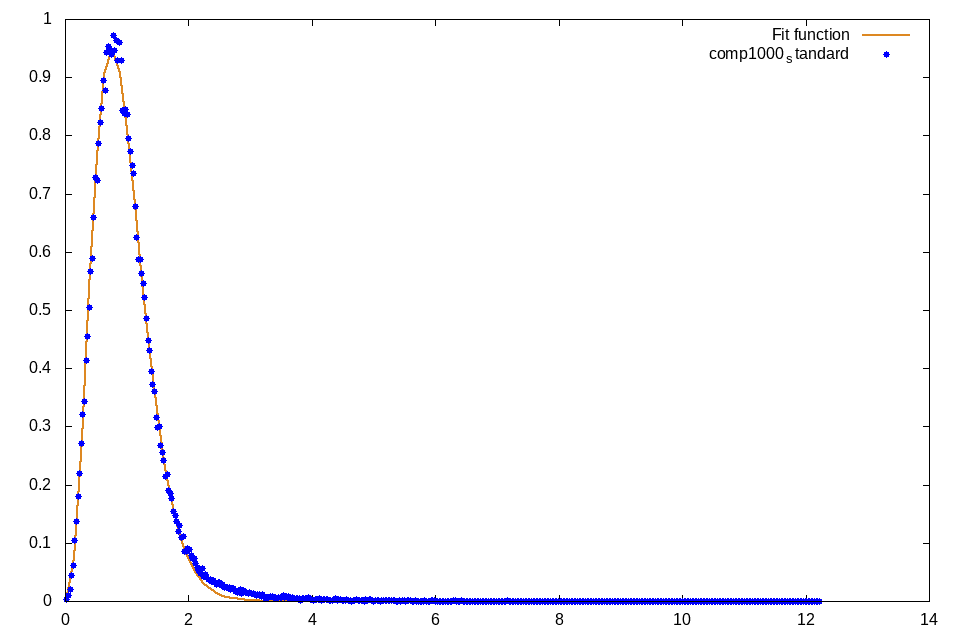
\includegraphics[scale=0.6]{./Comp_1000/hist_standard_fit.png}
	\caption{Results for hermitian matrix, dim = 1000, standard spacings.}
	\label{figure_lambdas}
\end{figure}


The fit results are the following.

\begin{table}[H]
	\centering
	\begin{tabular}{|c|c|c|}
		
		\hline
	
		a			& 15.10	& \\
		$\alpha$	& 2.641	& \\
		b			& 2.917	& \\
		$\beta$		& 1.297	& \\
		
		\hline
		
	\end{tabular}
\end{table}

\newpage

\begin{figure}[H]
	\centering
	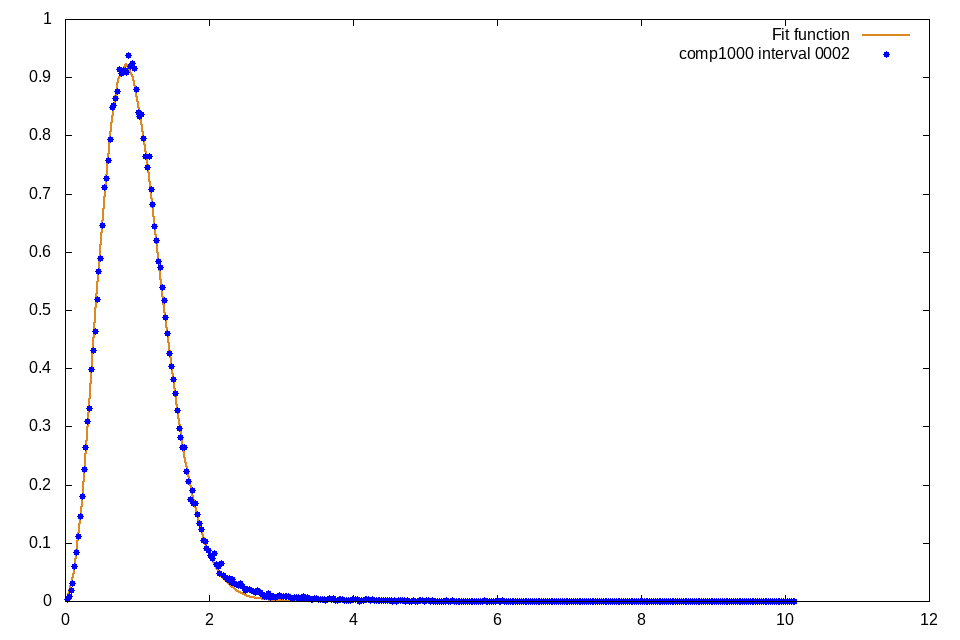
\includegraphics[scale=0.6]{./Comp_1000/hist_interval_0500_fit.png}
	\caption{Results for hermitian matrix, dim = 1000, spacings = N/2 = 500.}
	\label{figure_lambdas}
\end{figure}


The fit results are the following.

\begin{table}[H]
	\centering
	\begin{tabular}{|c|c|}
		
		\hline

		a			& 4.901	\\
		$\alpha$	& 2.189	\\
		b			& 1.731	\\
		$\beta$		& 1.693	\\
		
		\hline
		
	\end{tabular}
\end{table}

\newpage

\begin{figure}[H]
	\centering
	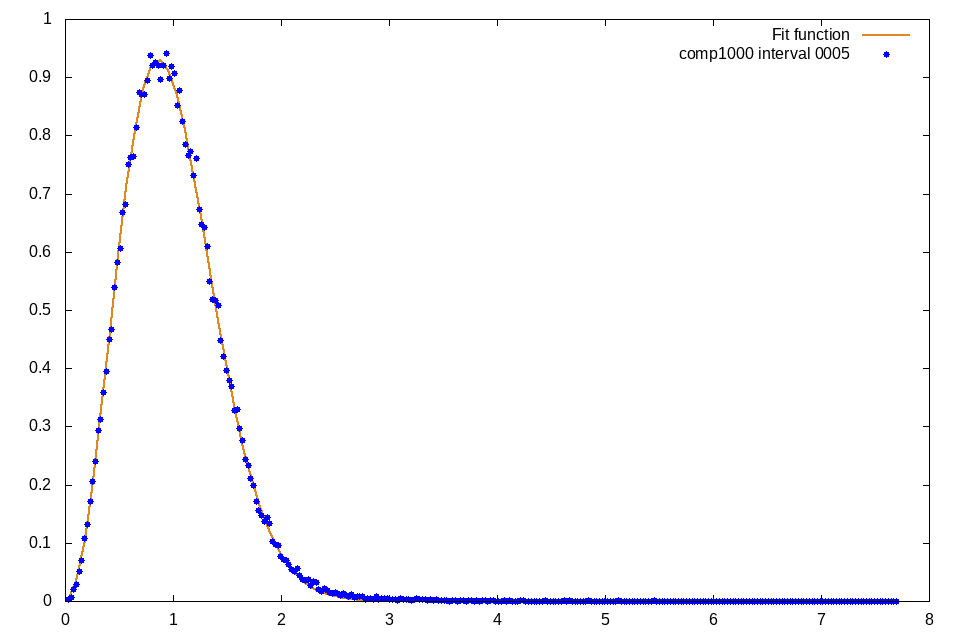
\includegraphics[scale=0.6]{./Comp_1000/hist_interval_0200_fit.png} 
	\caption{Results for hermitian matrix, dim = 1000, spacings = N/5 = 200.}
	\label{figure_lambdas}
\end{figure}

The fit results are the following.

\begin{table}[H]
	\centering
	\begin{tabular}{|c|c|}
		
		\hline
		     
		a			& 3.724	\\
		$\alpha$	& 2.052	\\
		b			& 1.4308	\\
		$\beta$		& 1.880 \\
		
		\hline
		
	\end{tabular}
\end{table}

\newpage

\begin{figure}[H]
	\centering
	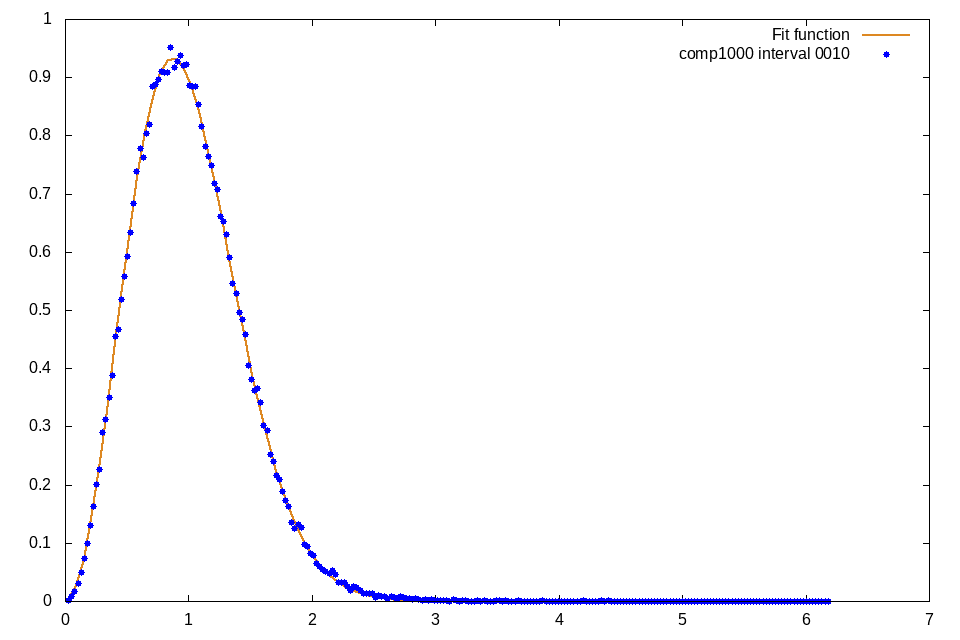
\includegraphics[scale=0.6]{./Comp_1000/hist_interval_0100_fit.png} 
	\caption{Results for hermitian matrix, dim = 1000, spacings = N/10 = 100.}
	\label{figure_lambdas}
\end{figure}

\begin{table}[H]
	\centering
	\begin{tabular}{|c|c|}
		
		\hline
		
		a			& 3.504	\\
		$\alpha$	& 2.027	\\
		b			& 1.362	\\
		$\beta$		& 1.929	\\
		
		\hline
		
	\end{tabular}
\end{table}

\newpage

\begin{figure}[H]
	\centering
	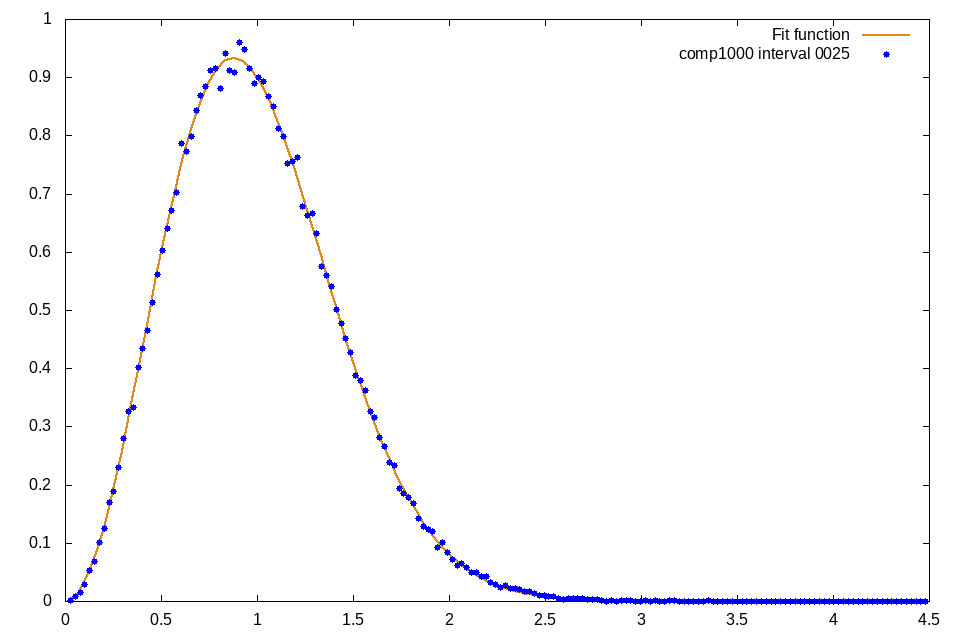
\includegraphics[scale=0.6]{./Comp_1000/hist_interval_0040_fit.png} 
	\caption{Results for hermitian matrix, dim = 1000, spacings = N/25 = 40.}
	\label{figure_lambdas}
\end{figure}

\begin{table}[H]
	\centering
	\begin{tabular}{|c|c|}
		
		\hline
    
		a			& 3.432	\\
		$\alpha$	& 2.021	\\
		b			& 1.338	\\
		$\beta$		& 1.943	\\
		
		\hline
		
	\end{tabular}
\end{table}

\newpage

\begin{figure}[H]
	\centering
	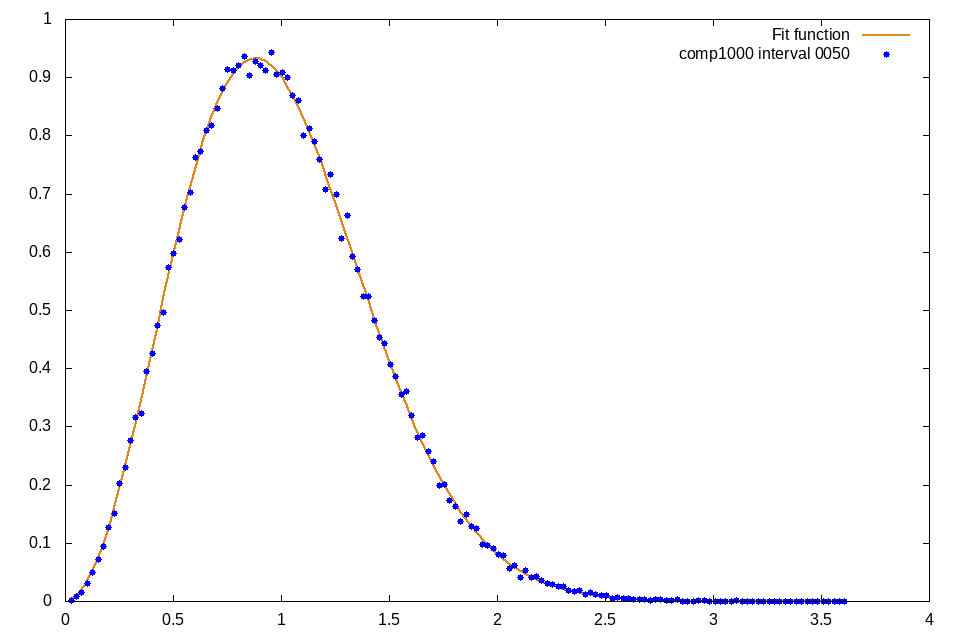
\includegraphics[scale=0.6]{./Comp_1000/hist_interval_0020_fit.png} 
	\caption{Results for hermitian matrix, dim = 1000, spacings = N/50 = 20.}
	\label{figure_lambdas}
\end{figure}

\begin{table}[H]
	\centering
	\begin{tabular}{|c|c|}
		
		\hline
   
		a			& 3.373	\\
		$\alpha$	& 2.013	\\
		b			& 1.340	\\
		$\beta$		& 1.955	\\
		
		\hline
		
	\end{tabular}
\end{table}

\newpage

\begin{figure}[H]
	\centering
	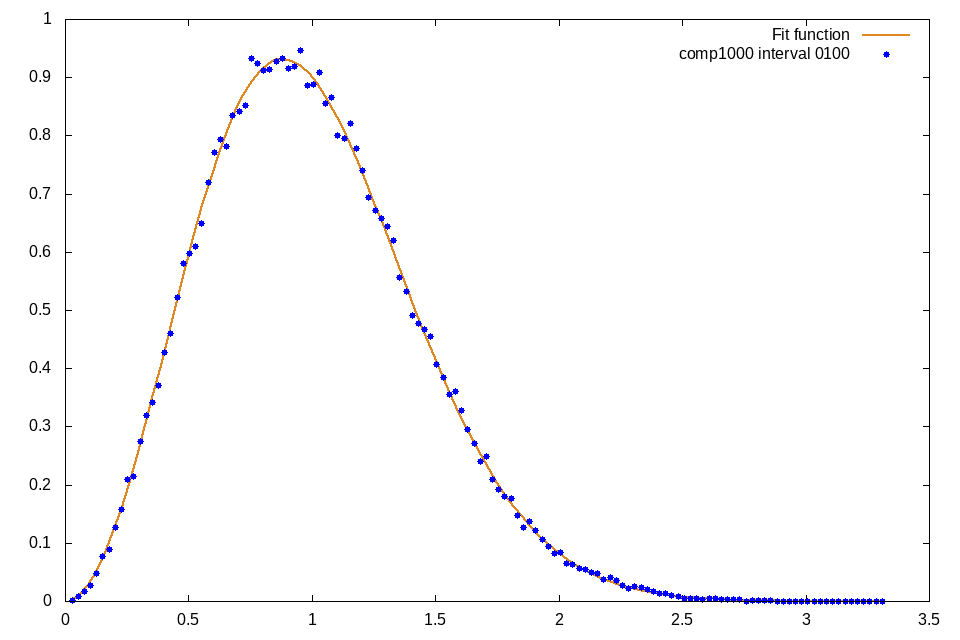
\includegraphics[scale=0.6]{./Comp_1000/hist_interval_0010_fit.png} 
	\caption{Results for hermitian matrix, dim = 1000, spacings = N/100 = 10.}
	\label{figure_lambdas}
\end{figure}

\begin{table}[H]
	\centering
	\begin{tabular}{|c|c|}
		
		\hline
		 
		a			& 3.381	\\
		$\alpha$	& 2.018	\\
		b			& 1.322	\\
		$\beta$		& 1.951	\\
		
		\hline
		
	\end{tabular}
\end{table}

\newpage

\begin{figure}[H]
	\centering
	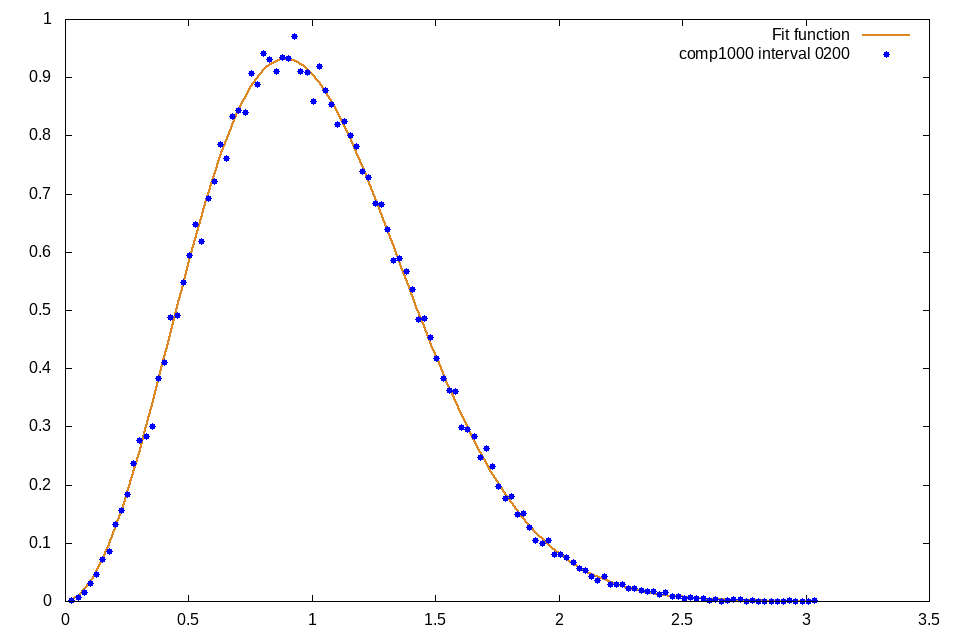
\includegraphics[scale=0.6]{./Comp_1000/hist_interval_0005_fit.png} 
	\caption{Results for hermitian matrix, dim = 1000, spacings = N/200 = 5.}
	\label{figure_lambdas}
\end{figure}

\begin{table}[H]
	\centering
	\begin{tabular}{|c|c|}
		
		\hline
		   
		a			& 3.095	\\
		$\alpha$	& 1.982	\\
		b			& 1.227	\\
		$\beta$		& 2.027	\\
		
		\hline
		
	\end{tabular}
\end{table}


% REAL 1000

\newpage

.

\vspace{10cm}

The fit for standard spacings did not converged in gnuplot.

\newpage

\begin{figure}[H]
	\centering
	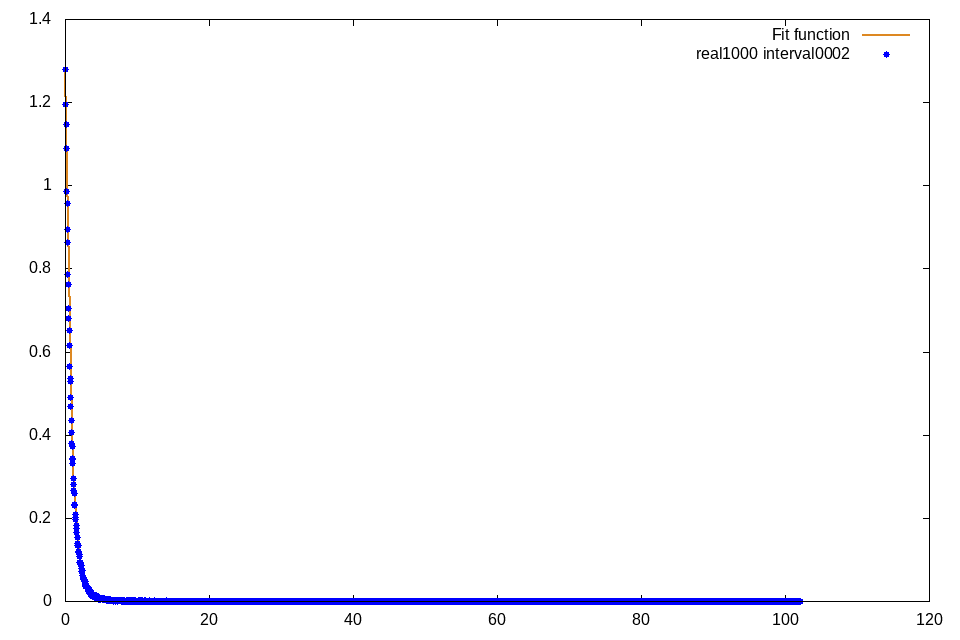
\includegraphics[scale=0.6]{./Real_1000/hist_interval_0500_fit.png}
	\caption{Results for real matrix, dim = 1000, spacings = N/2 = 500.}
	\label{figure_lambdas}
\end{figure}


The fit results are the following.

\begin{table}[H]
	\centering
	\begin{tabular}{|c|c|}
		
		\hline
   
		a			& 1.521	\\
		$\alpha$	& 0.032	\\
		b			& 1.520	\\
		$\beta$		& 0.854	\\
		
		\hline
		
	\end{tabular}
\end{table}

\newpage

\begin{figure}[H]
	\centering
	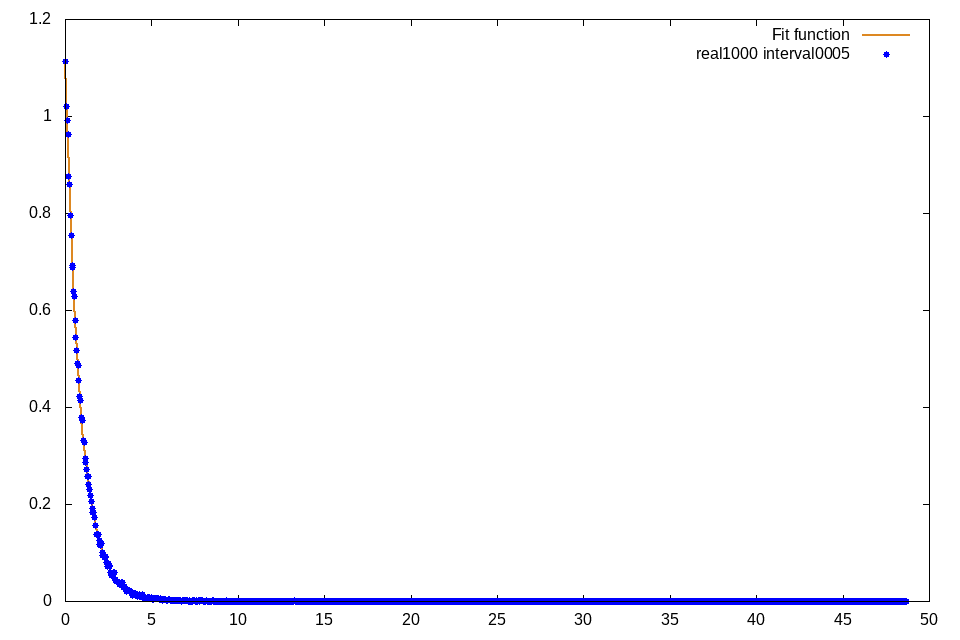
\includegraphics[scale=0.6]{./Real_1000/hist_interval_0200_fit.png} 
	\caption{Results for real matrix, dim = 1000, spacings = N/5 = 200.}
	\label{figure_lambdas}
\end{figure}

The fit results are the following.

\begin{table}[H]
	\centering
	\begin{tabular}{|c|c|}
		
		\hline
    
		a			& 1.185	\\
		$\alpha$	& 0.0089	\\
		b			& 1.211	\\
		$\beta$		& 1.922	\\
		
		\hline
		
	\end{tabular}
\end{table}

\newpage

\begin{figure}[H]
	\centering
	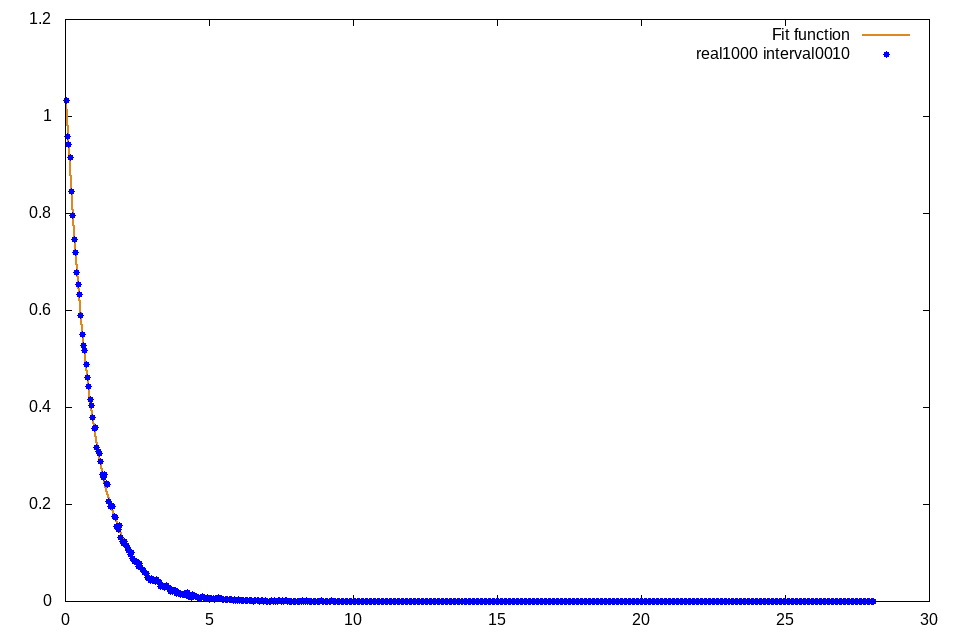
\includegraphics[scale=0.6]{./Real_1000/hist_interval_0100_fit.png} 
	\caption{Results for real matrix, dim = 1000, spacings = N/10 = 100.}
	\label{figure_lambdas}
\end{figure}

\begin{table}[H]
	\centering
	\begin{tabular}{|c|c|}
		
		\hline
 
		a			& 1.093	\\
		$\alpha$	& 0.0074	\\
		b			& 1.108	\\
		$\beta$		& 0.952	\\
		
		\hline
		
	\end{tabular}
\end{table}

\newpage

\begin{figure}[H]
	\centering
	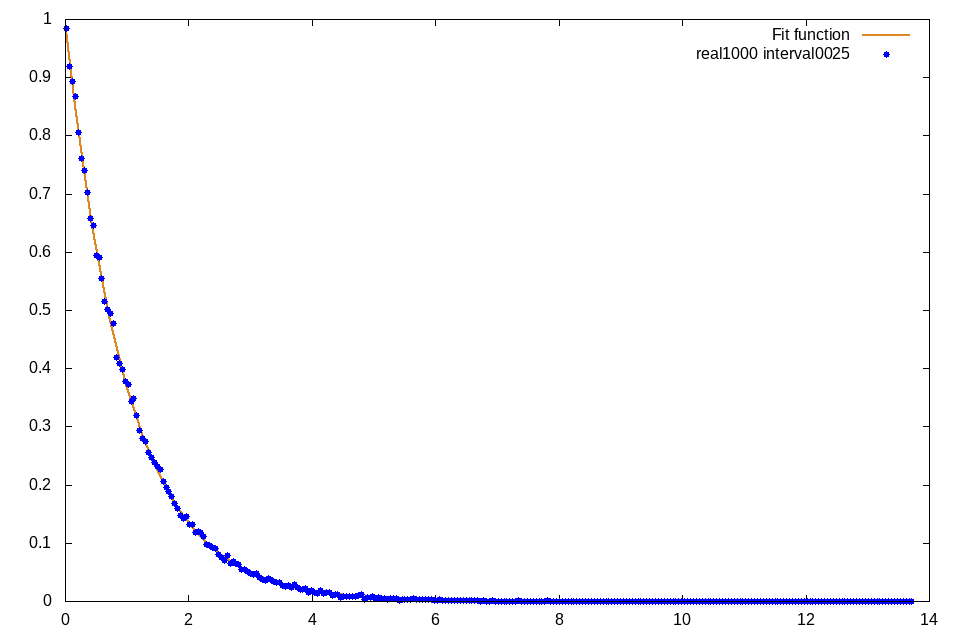
\includegraphics[scale=0.6]{./Real_1000/hist_interval_0040_fit.png} 
	\caption{Results for real matrix, dim = 1000, spacings = N/25 = 40.}
	\label{figure_lambdas}
\end{figure}

\begin{table}[H]
	\centering
	\begin{tabular}{|c|c|}
		
		\hline

		a			& 0.9818	\\
		$\alpha$	& -0.0059	\\
		b			& 0.979	\\
		$\beta$		& 1.012	\\
		
		\hline
		
	\end{tabular}
\end{table}

\newpage

\begin{figure}[H]
	\centering
	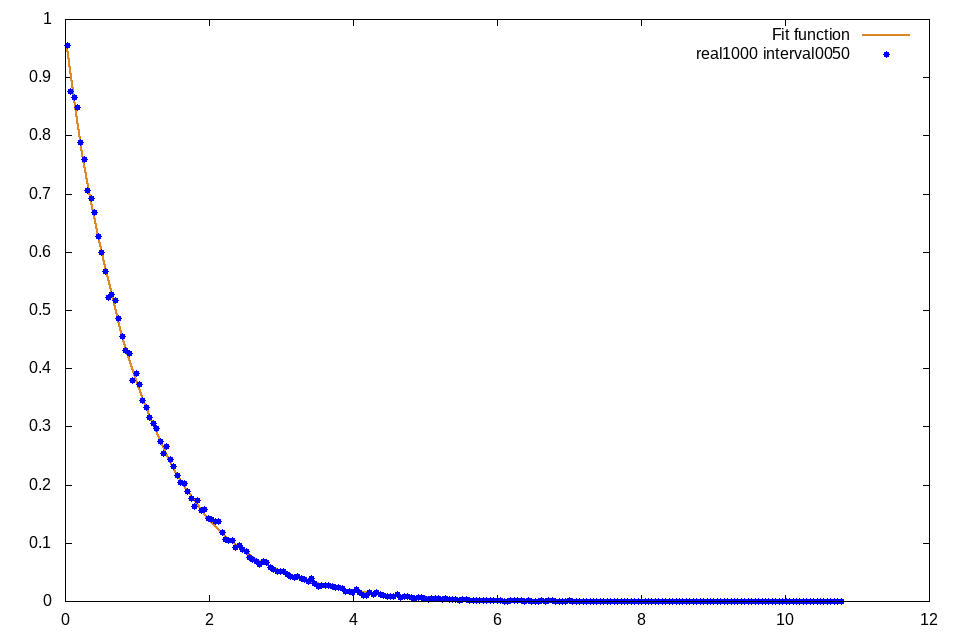
\includegraphics[scale=0.6]{./Real_1000/hist_interval_0020_fit.png} 
	\caption{Results for real matrix, dim = 1000, spacings = N/50 = 20.}
	\label{figure_lambdas}
\end{figure}

\begin{table}[H]
	\centering
	\begin{tabular}{|c|c|}
		
		\hline

		a			& 0.916	\\
		$\alpha$	& -0.0143	\\
		b			& 0.894	\\
		$\beta$		& 1.062	\\
		
		\hline
		
	\end{tabular}
\end{table}

\newpage

\begin{figure}[H]
	\centering
	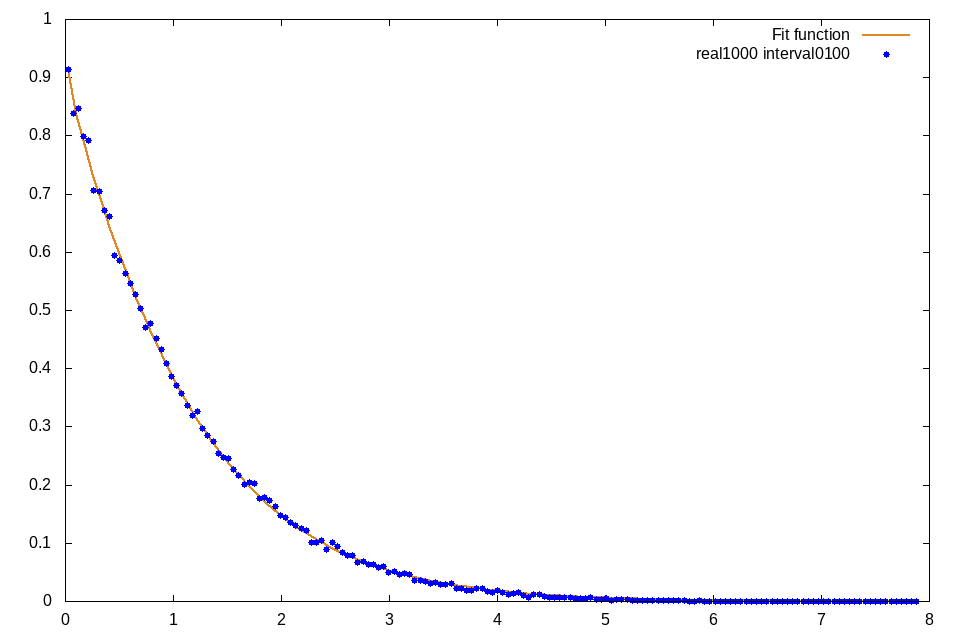
\includegraphics[scale=0.6]{./Real_1000/hist_interval_0010_fit.png} 
	\caption{Results for real matrix, dim = 1000, spacings = N/100 = 10.}
	\label{figure_lambdas}
\end{figure}

\begin{table}[H]
	\centering
	\begin{tabular}{|c|c|}
		
		\hline

		a			& 0.829	\\
		$\alpha$	& -0.0288	\\
		b			& 0.769	\\
		$\beta$		& 1.151	\\
		
		\hline
		
	\end{tabular}
\end{table}

\newpage

\begin{figure}[H]
	\centering
	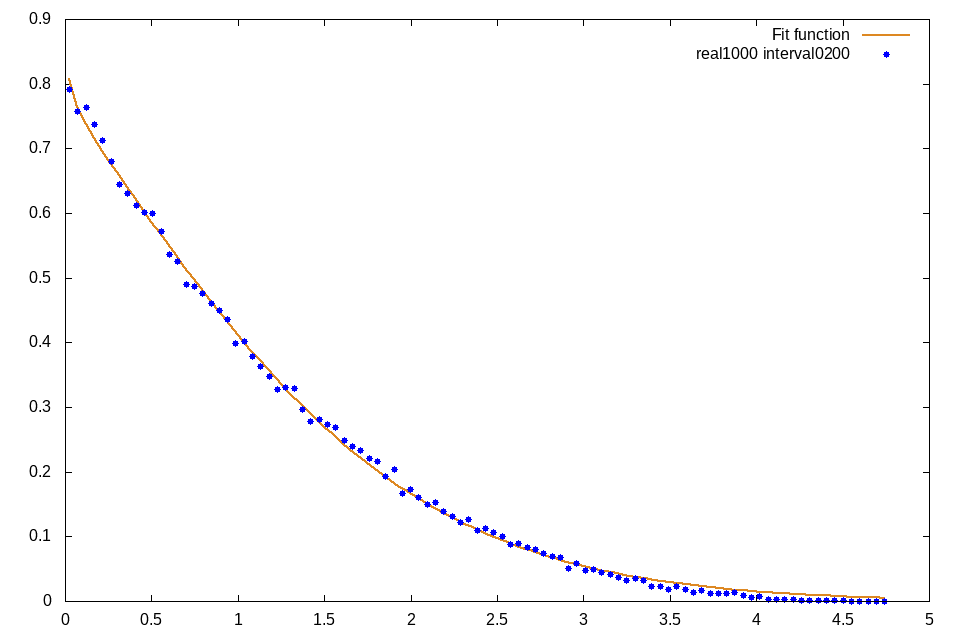
\includegraphics[scale=0.6]{./Real_1000/hist_interval_0005_fit.png} 
	\caption{Results for real matrix, dim = 1000, spacings = N/200 = 5.}
	\label{figure_lambdas}
\end{figure}

\begin{table}[H]
	\centering
	\begin{tabular}{|c|c|}
		
		\hline
		a			& 0.689	\\
		$\alpha$	& -0.043	\\
		b			& 0.515	\\
		$\beta$		& 1.435	\\
		
		\hline
		
	\end{tabular}
\end{table}

\vspace{2cm}

For what concerns dim=1500 and dim=2000 results, they are similar to those shown above.\\ \\ \\ \\
Looking at hermitian results, one can notice that they improve (i.e. become closer to theoretical results) with spacings improving, thus considering smaller eigenvalues interval to evaluate local spacings.

\newpage

\section*{Self-evaluation}
In this task I learned how to generate random distributed numbers using Fortran and how to use them to generate random matrices; how to write a simple sort routine, how to handle arguments in Python scripts, bash scripts and also in gnuplot scripts. Also, I tried to automatize as much as possible the whole task, saving and storing data results in a clear way so to retrieve them if needed.\\ \\
My work can be improved in many ways. First of all, the analysis is only partial and it is done only "by glance": a more seriuos one should be done, considering standard deviation on parameters esteems and verify the compatibility with theoretical results. Images also should be improved, inserting more information about axes. For this task I did not dealt properly with these features because I preferred to spend more time on automatizing the task using a single Python script.\\ \\
Some issues arose also using Gnuplot: since it uses an iterative method to fit, it sometimes failed fitting due to the bad parameters initialization. They should be initialized properly for every fit which is taken into account, but this requires time to be done properly.

\end{document}